\chapter{Analysis}

\section{Selection Cuts}
\label{selectioncuts}

This section describes data used for the single top quark analysis as well as all selection cuts applied to the data and Monte Carlo samples. The goal of the trigger and selection cuts is to retain as many signal events as possible while reject mis-measured evens and events not consistent with the single top final state. As described in Section~\ref{electroweaktopquark}, the final state for single top quark events is (1) lepton, (1) neutrino (seen as missing transverse energy), and (2) b quarks for $s$-channel or at least (1) b quark for the $t$-channel and (1) light quark. Due to higher order affects, the events might acquire other light flavor quarks or gluons from initial state or final state iation.

Section~\ref{datasample} describes the triggers used the single top analysis to select interesting events at runtime The efficiency of the trigger for single top Monte Carlo events is also reported. Section~\ref{dataquality} describes the criteria used to ensure the $\dzero$~detector was recording physics quality data when the trigger was allowed to select events. Section~\ref{objectselection} details the selection cuts applied to all physics objects in the event. Signal efficiencies for both the $s$ and $t$-channel are reported for each cut.

\subsection{Data Sample}
\label{datasample}

\subsection{Reconstructed Object Trigger Efficiencies}
\label{turnoncurves}

Trigger term efficiencies must be measured for each trigger level with respect to all reconstructed objects in the event that could cause a trigger selection. For triggers used to collect top quark events, this requires efficiencies for electron, muon, and jet trigger terms. 

 Fig.~\ref{muontrigeff} shows the Level1, Level2, and Level3 trigger efficiencies for muon trigger terms important to top quark triggers and Fig.~\ref{electrontrigeff} shows similar plots for electron trigger terms. A more detailed description of the trigger requirements for the single top quark analysis, including trigger definitions, can be found in Section.~\ref{datasample}


\begin{figure}[!h!tbp]
\begin{center}
\includegraphics[width=0.45\textwidth]{eps/Reco/l1atxx.eps}
\includegraphics[width=0.45\textwidth]{eps/Reco/l1atlx.eps}
\includegraphics[width=0.45\textwidth]{eps/Reco/l2m0.eps}
\includegraphics[width=0.45\textwidth]{eps/Reco/l3l3.eps}
\end{center}
\vspace{-0.1in}
\caption[muontrigeff]{Muon trigger efficiencies as a function $\eta$-$\phi$ for four commonly used trigger terms: level1 tight muon scintillator hit (top left), level1 tight muon scintillator with a loose wire hit (top right), level2 medium muon (bottom left), and level3 loose muon with $p_{T}>3$~GeV.}
\label{muontrigeff}
\end{figure}


\subsection{Data Quality}
\label{dataquality}

\subsection{Physics Object Selection}
\label{objectselection}

The following subsections describe the selection cuts applied to the data and Monte Carlo events. The goal of the selection cuts is retain high quality physics objects while rejecting fake objects created by detector noise additional low energy physics processes in the event.

\subsubsection{Muon Selection}
\label{muonselection}

To be consistent with a single top quark production and decay, the event must have at most one muon that is isolated as described in Section~\ref{muonreco} with $p_{T}>18$~GeV and $|\eta^{det}|<2$. The track associated with muon is required to less than 1 cm from primary interaction vertex along the $z$~direction. To reject $Z\rightarrow\mu\mu$+jets and $\ttbar$ backgrounds, a veto on muons with $p_{T}>15$~GeV with no requirement on isolation is applied. Events which pass these criteria also veto electrons with $p_{T}>15$ and $|\eta^{det}|<1.1$ to ensure orthogonality of search channels.



\begin{table}[!h!tbp]
\begin{center}
\begin{tabular}{c||ccc|ccc}
\multicolumn{7}{c}
{\underline{$s$ and $t$-channel Muon Selection Cut Efficiencies}} \\
& \multicolumn{3}{c}{\underline{$s-channel}}
& \multicolumn{3}{c}{\underline{$t-channel}} \\
Generation	&	Flavor	&	Charge	&	Mass [MeV]				&	Flavor					&	Charge	&	Mass [MeV]	\\
\hline
1	&	Up (u)		&	+$\frac{2}{3}$e	&	1.5 to 3.0					&	Electron (e)				&	-e		&	0.511	\\
	&	Down (d)		&	-$\frac{1}{3}$e	&	3 to 7					&	Electron neutrino ($\nu_{e}$)	&	0		&	$<$ 2.2 $\times$ $10^{-6}$	\\
\hline
2	&	Charm (c)		&	+$\frac{2}{3}$e	&	1.25 $\times$ $10^{3}$		&	Muon ($\mu$)				&	-e		&	105.7	\\
	&	Strange (s)	&	-$\frac{1}{3}$e	&	90						&	Muon neutrino ($\nu_{\mu}$)	&	0		&	$<$ 1.7 $\times$ $10^{-4}$	\\
\hline
3	&	Top (t)		&	+$\frac{2}{3}$e	&	171.4 $\times$ $10^{3}$		&	Tau ($\tau$)				&	-e		&	1777		\\
	&	Bottom (b)		&	-$\frac{1}{3}$e	&	4.7 $\times$ $10^{3}$		&	Tau neutrino ($\nu_{\tau}$)	&	0		&	$<$ 15.5	\\
\end{tabular}
\vspace{-0.1 in}
\caption{Properties of the fundamental spin=$\frac{1}{2}$ fermions in the Standard Model}
\label{fermions}
\end{center}
\end{table}


\subsubsection{Electron Selection}
\label{electronselection}

Electrons are required have $p_{T}>15$~GeV and $|\eta^{det}|<1.1$ to be consistent with single top production. Similar to the muon selection, a veto is placed on additional electrons to reject $Z\rightarrow ee$+jets and $\ttbar$ backgrounds. The electron track is also required to pass within 1 cm of the primary interaction vertex along the $z$~direction. To provide orthogonality with the muon search channel, events that pass the electron selection criteria veto events which pass the muon selection criteria.

\subsubsection{Jet Selection}
\label{jetselection}

To maximize signal acceptance events are required to have between two and four fully corrected jets. The leading jet (highest $p_{T}$) must have $p_{T}>25$~GeV and $|\eta^{det}|<2.5$. The second jet (second highest $p_{T}$) must have $p_{T}>20$~GeV and $|\eta^{det}|<3.4$. All other jets in the event must have $p_{T}>15$~GeV and $|\eta^{det}|<3.4$.


\subsubsection{Missing $E_{T}$}
\label{missingetselection}

A large amount of missing transverse energy in an event can indicate the presence of a neutrino in the final state. All events are required to have at least $15$~GeV of $\met$ that is corrected for jets with JES applied, including jets with semi-leptonic decays, and corrected for high $p_{T}$ electrons or muons in the event.

\subsubsection{Vertex Selection}
\label{vertexselection}

All events are required to have one and only one one hard-scatter vertex as defined in Section~\ref{pvreco}.

\subsubsection{b-Jet Selection}
\label{bjetselection}

Both $s$-channel and $t$-channel single top quark events have at least one b quark in the final state so all events must have at least one $B$-jet as identified by the neural network tagging algorithm described in Section~\ref{bidreco}.

\subsubsection{Mis-measured event rejection}
\label{misidselection}

There are several selection cuts applied to reduce or eliminate either mis-measured events or events with similar event topology as single top, but originating from a high cross section QCD multi-jet process. The first cut applied is to remove events where the muon track momentum has been badly measured, which can cause an imbalance in the missing transverse energy measurement. All events are required to have ME$_{T}<200$~GeV. The next cut applied is to allow at most three "noise" jets. A noise jet is a jet that fails one of the criteria specified in Section~\ref{jetreco} and is not matched to an electromagnetic cluster. These jets are not included in the $\met$ however are allowed to exist simultaneously in the event. It has been observed that allowing more than three noise jets beings to alter the $p_{T}$ and $\eta$~distributions of other jets in the event. The final set of cuts applied to remove unwanted events are "triangle cuts", which are cuts between an the difference in $\phi$ between an object and the $\met$ versus the $\met$ itself. An example of triangle cut is shown in Fig.~\ref{triangleexample}. Three sets of triangle cuts are applied to the data and Monte Carlo events and shown in the bullets below.

\begin{itemize}
\item Electron Triangle Cuts: $|\Delta\phi(\rm{e},$ME$_{T})|$~vs.~$\met$
   \begin{itemize}
   \item $0<|\Delta\phi|<2$~ when ME$_{T} = 0$~GeV, and $0<$ME$_{T}<40$~GeV when $|\Delta\phi| = 0$
   \item $0<|\Delta\phi|<1.5$~ when ME$_{T} = 0$~GeV, and $0<$ME$_{T}<50$~GeV when $|\Delta\phi| = 0$
   \item  $2<|\Delta\phi|<\pi$~ when ME$_{T} = 0$~GeV, and $0<$ME$_{T}<24$~GeV when $|\Delta\phi| = \pi$
   \end{itemize}
\item Muon Triangle Cuts: $|\Delta\phi(\mu,$ME$_{T})|$~vs.~$\met$
   \begin{itemize}
   \item  $0<|\Delta\phi|<1.1$~ when ME$_{T} = 0$~GeV, and $0<$ME$_{T}<80$~GeV when $|\Delta\phi| = 0$
   \item  $0<|\Delta\phi|<1.5$~ when ME$_{T} = 0$~GeV, and $0<$ME$_{T}<50$~GeV when $|\Delta\phi| = 0$
   \item $2.5<|\Delta\phi|<\pi$~ when ME$_{T} = 0$~GeV, and $0<$ME$_{T}<30$~GeV when $|\Delta\phi| = \pi$
   \end{itemize}
\item Leading Jet Triangle Cut: $|\Delta\phi(\rm{Jet_{1}},$ME$_{T})|$~vs.~$\met$
   \begin{itemize}
   \item $1.5<|\Delta\phi|<\pi$~ when ME$_{T} = 0$~GeV, and $0<$ME$_{T}<35$~GeV when $|\Delta\phi| = \pi$
   \end{itemize}
\end{itemize}



\begin{figure}[!h!tbp]
\begin{center}
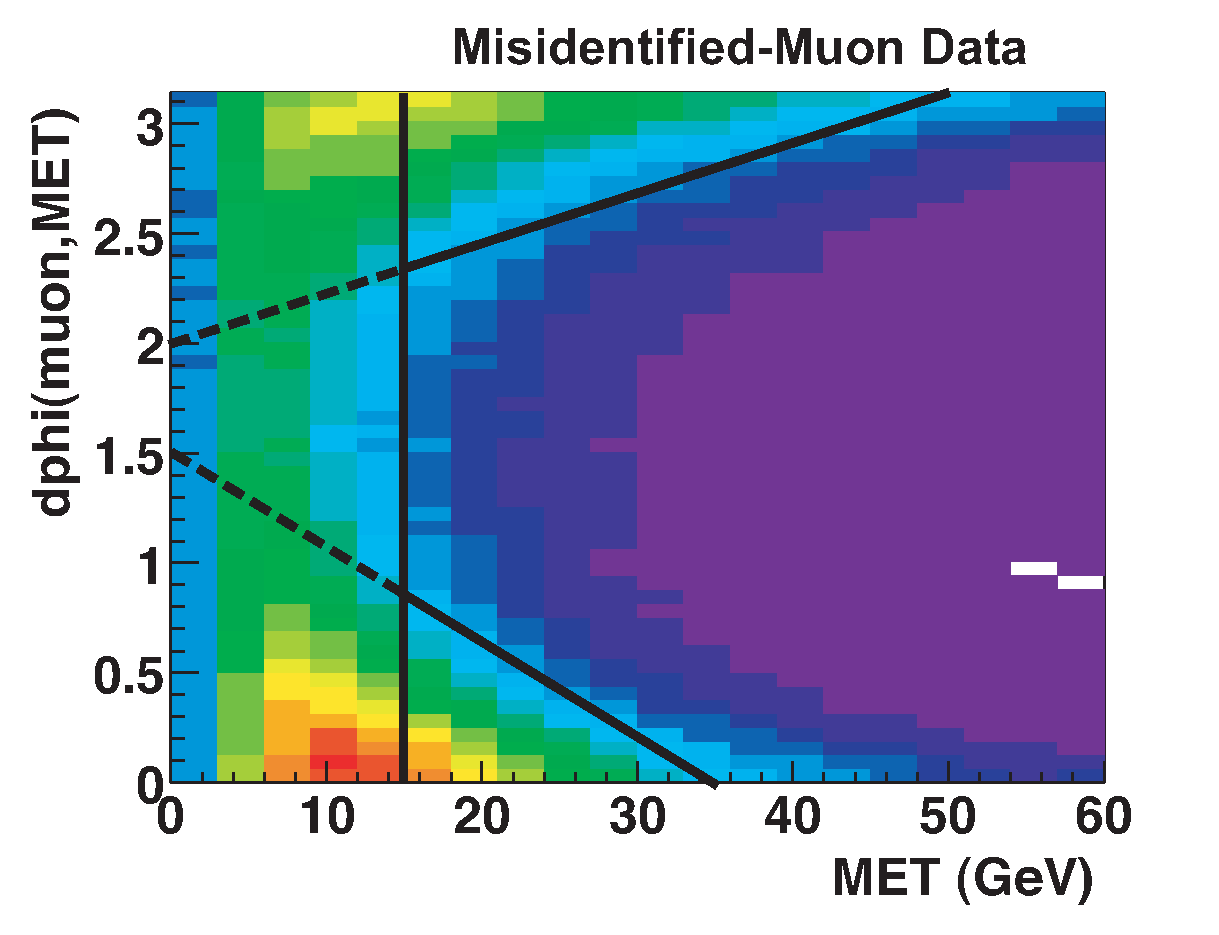
\includegraphics[width=0.5\textwidth]{eps/Reco/TriangleExample.eps}
\end{center}
\vspace{-0.1in}
\caption[triangleexample]{Example triangle cut between a muon and the $\met$. Events which fall inside the triangles are removed the final data sample. The black line at $\met$~GeV indicates the standard $\met$ selection.} 
\label{triangleexample}
\end{figure}



\section{Background Modelling}
\subsection{W/Z Boson + Jets}
\subsection{\ttbar}
\subsection{Multijet}

\section{Background Normalization}
\subsection{Matrix Method: Normalizing W+jets and Multijet Backgrounds}
\subsection{\ttbar}

\section{Event Yields}
\subsection{Signal Acceptance}
\subsection{Background Yields}
